\documentclass{article}
\usepackage[accepted]{icml2018}
\usepackage{graphicx}

\icmltitlerunning{Neural Network Pruning Techniques}

\begin{document}

\twocolumn[
\icmltitle{E0:270 - Machine Learning - Neural Network Pruning Techniques}

\icmlsetsymbol{equal}{*}

\begin{icmlauthorlist}
\icmlauthor{Braunstein, Cameron}{dep2}
\icmlauthor{Nair, Abhishek}{dep1}
\icmlauthor{Shaw, Vishal}{dep3}
\end{icmlauthorlist}

\icmlaffiliation{dep1}{Department of Electronic System Engineering, Indian Institute of Science, Bangalore}
\icmlaffiliation{dep2}{Mathematics Department, Indian Institute of Science, Bangalore}
\icmlaffiliation{dep3}{Electrical Communication Engineering, Indian Institute of Science, Bangalore}

\icmlcorrespondingauthor{Braunstein, Cameron}{comeronb@iisc.ac.in}
\icmlcorrespondingauthor{Nair, Abhishek}{abhisheknair@iisc.ac.in}
\icmlcorrespondingauthor{Shaw, Vishal}{vishalshaw@iisc.ac.in}

\icmlkeywords{neural network, pruning, machine learning}

\vskip 0.3in
]

\printAffiliationsAndNotice{}

\begin{abstract}
This project investigated various methods of pruning a neural network. After a literature survey on various algorithms, we finalized two distinct approaches: Layered Optimal Brain Surgeon (L-OBS) and Neural Network Pruning by Significance (N2PS) for implementation. The findings were clear that L-OBS works well for larger networks compared to N2PS algorithm in terms of pruning. We would want to explore a novel algorithm for pruning based on our findings. 
\end{abstract}

\section{Motivation}
\label{Motivation}
Deep neural networks are flexible function approximators that have been very successful in a
broad range of tasks. They can easily scale to millions of parameters, which results in challenges to store and load the network. Additionally, large networks can overfit to training data and can even memorize random patterns \cite{Louizos17}. Neural network pruning seeks to remove unimportant weights from the network. This reduces the network's size in memory and can reduce overfitting. 
\section{Literature Review}
\label{Literature Review}
The Optimal Brain Surgeon algorithm (OBS) takes a pretrained network, and prunes weights based on their calculated effect on the error using a second order Taylor expansion of the error function, and adjusts the unpruned weights to compensate \cite{Hassibi93}. Layerwise OBS (L-OBS) simplifies the OBS algorithm by only considering a weight's effect on local error. It has been demonstrated that any increase in the total error from pruning a weight is reasonably bounded above by the corresponding increase in local error by pruning that weight \cite{Dong17}. Thus L-OBS approximates OBS and is more computationally feasible.

The N2PS algorithm optimizes the structure of neural networks by pruning neurons from each layer. The pruning is done based on the significance of each neuron, which is calculated by getting the normalized average value of neurons for each layer.This is followed by comparing each neuron value with the normalized average value i.e. the significant value. The neurons which have less than the significant value is pruned and the network is retrained for accuracy \cite{Augasta11}.

L0 regularization is a pruning technique which can be executed during the networks' initial training phase. The L0 norm of the weights is non differentiable. However by smoothing the expected L0 norm with continuous distributions with hard nonlinearity, it is possible to maintain exact zeros in the pruned weights while still allowing for efficient gradient based optimization \cite{Louizos17}. 

The Deep Compression method combines pruning with other size reduction techniques. First, a trained network is pruned by magnitude, ie, weights with an absolute value below a threshold are dropped. Next, weight values are quantized, so that multiple connections share the same weight, thus only the effective weights and the indices need to be stored. Finally, Huffman coding is applied to take advantage of the biased distribution of effective weights \cite{Han15}.

\section{Experiment Description}
\label{Experiment Description} We trained a 784-300-100-10 feed foward neural network with L2 regularization to classify the MNIST dataset. There were 266200 prunable weights in total. We then tested several pruning algorithms on the network. 

In our first experiment, we ran N2PS algorithm on this network. We implemented the algorithm where instead of pruning the neurons, we assigned the weights associated with the pruned neuron as zero.

We then compared these approaches, which could be run until they reached a compression ratio of 0. We implemented magnitude based weight pruning as a control. Against this, we ran a simplified version of the L-OBS algorithm, which recalculated the inverse Hessian only after every 2000 pruned weights. We also ran this simplified L-OBS algorithm, with 3 iterations of retraining after every 2000 pruned weights and then a recalculation of the inverse Hessian. In the original L-OBS algorithm, the inverse Hessian is recalculated after every pruned weight. However this change was made out of computational necessity.

\section{Preliminary Results}
\label{Preliminary Results}

\begin{center}
\textbf{N2PS on smaller data set (Literature Survey data)}
\begin{tabular}{|c|c|c|c|} 
\hline
\multicolumn{4}{|c|}{Accuracy} \\
\hline
Dataset&Architecture&Pre Pruning&Post Pruning\\
\hline
Iris & 4-10-3 & 97.3\% & 98.67\%  \\ 
Cancer & 9-10-2 & 95.4\% & 97.1\%  \\ 
Ionosphere & 34-10-2 &91.4\% & 94.9\% \\
\hline
\end{tabular}
\end{center}
\vspace*{-0.28cm}
The N2PS algorithm as per literature performed the best for smaller networks like iris-dataset, breast-cancer, ionosphere etc. These dataset are of the order of 50-10-2 network architecture. For these architecture, N2PS pruning helped improve the accuracy of the network.
\begin{center}
\textbf{N2PS on MNIST (Based on our Experiment)}

 \begin{tabular}{|c|c|c|c|}
 \hline
 \multicolumn{4}{|c|}{Accuracy} \\
 \hline
Dataset & Architecture & Pre Pruning & Post Pruning  \\
 \hline
MNIST  & 784-300-100-10 & 94.6\% & 89.98\%  \\ 
 \hline
 \end{tabular}
\end{center}

 Results which were obtained on 748-300-100-10 network using N2PS seemed to reduce the accuracy .
With smaller architecture, the distinctiveness of a contributing neuron would be higher compared to a larger network where lot of the contributing neurons might get pruned if they lie just below the threshold value. Hence N2PS algorithm seem to work well on smaller network. 

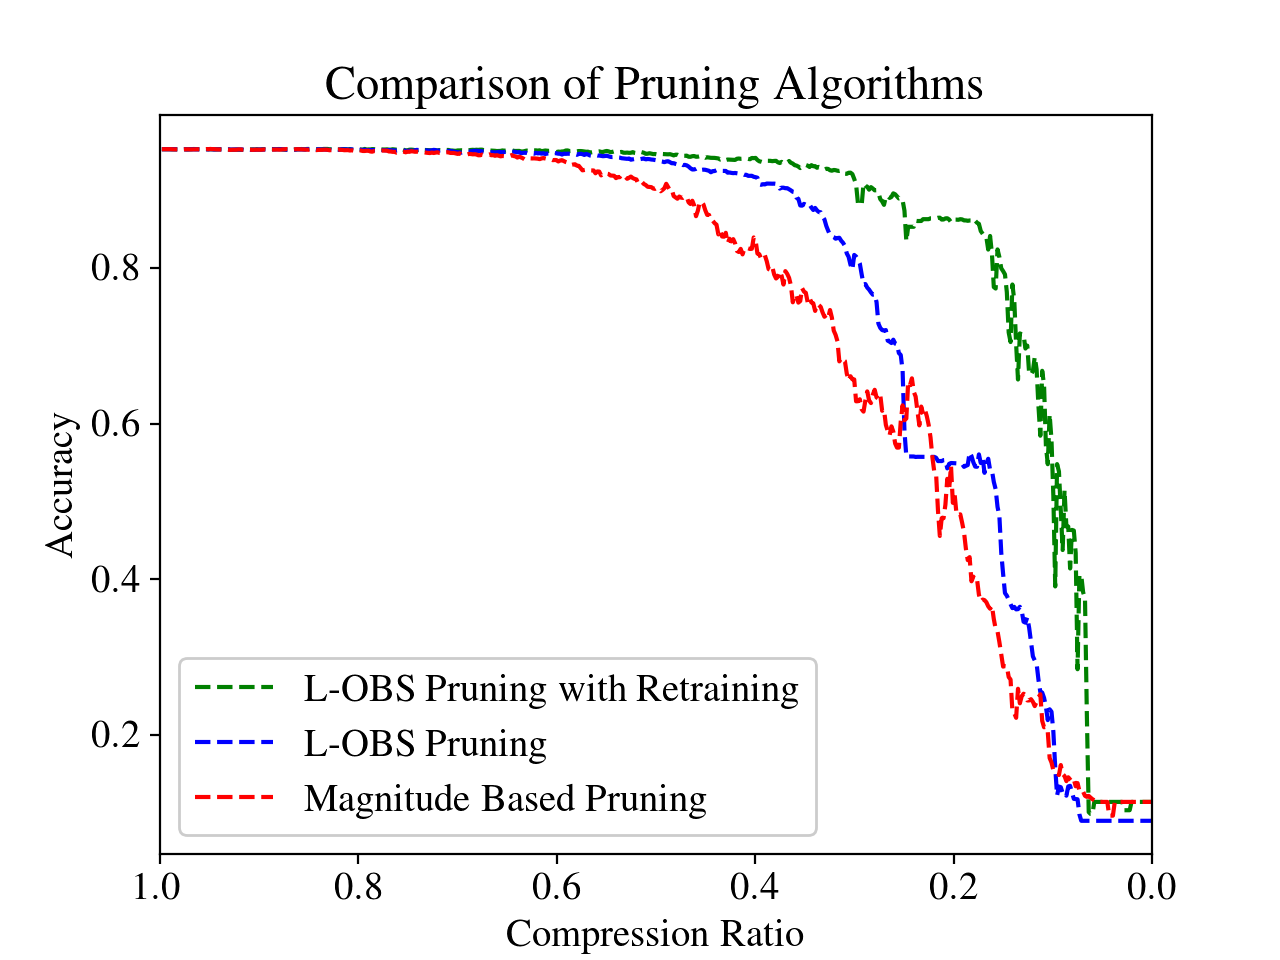
\includegraphics[scale=0.65]{Comparison}

Our control, the Magnitude Based Pruning, dropped in accuracy the fastest, followed by our simplified L-OBS algorithm and then simplified L-OBS with retraining. The L-OBS with retraining graph is particularly jagged, as retraining every 2000 prunings resulted in spikes of accuracy, particularly as the network became more sparse. Interestingly, all algorithms stayed closed to their initial test accuracy until a compression ratio of approximately 0.6. This suggests that the network has redundancies which can be eliminated before training begins.

From the results, we clearly see that N2PS seems to struggle with bigger than 100 neuron network. On the other hand L-OBS seems to be a stable and viable option for neural network pruning for larger networks. 

\section{Future Work}
\label{Future Work}

We hope to combine several of our tested algorithms to see if we can achieve even better compression without loss in accuracy. We also hope to explore L0 regularization in depth. 

One interesting algorithm we would want to explore is to try and optimize L0 regularization and implement it layer wise just like we have seen in case of OBS.

%%%%%%%%%%%%%%%%%%%%%%%%%%%%%%%%%%%%%%%%%%%%%%%%%%%%%%%%%%%%%%%%%%%%%%%%%%%%%%%

\newpage

\bibliography{biblio}
\bibliographystyle{icml2018}


\end{document}